\documentclass[11pt]{article}
\usepackage[english]{babel}
\usepackage{array} % for better arrays (eg matrices) in maths
\usepackage{booktabs} %Tablas quedan mejor
\usepackage{vmargin} %M�rgenes
\usepackage{hyperref}
\usepackage[T1]{fontenc}
\setpapersize{A4}
\setmargins{2.5cm}       % margen izquierdo
{1.5cm}                        % margen superior
{16.5cm}                      % anchura del texto
{22.42cm}                    % altura del texto
{10pt}                           % altura de los encabezados
{1.5cm}                           % espacio entre el texto y los encabezados
{0pt}                             % altura del pie de p�gina
{2cm}                           % espacio entre el texto y el pie de p�gina

\usepackage[none]{hyphenat} %No corta palabras al final de las lineas
\usepackage{graphicx} %Im�genes
\usepackage{subfigure} % subfiguras
\graphicspath{{img/}} % Root for images
\usepackage{wrapfig}
\usepackage{siunitx} %Escribir n�meros y unidades
\usepackage{amsmath} %Mayor facilidad para escribir matrices y otros elementos matem�ticos
%\numberwithin{equation}{section} %En las ecuaciones se especifica tambi�n el cap�tulo
\usepackage{xcolor} %Colores (\color{})
\usepackage{lipsum}
\usepackage{topcapt}
\usepackage{parskip}
\usepackage{braket}
\usepackage{setspace}
\usepackage{listings}
\usepackage{graphicx}
\graphicspath{ {images/} }
\usepackage{float}
\usepackage{fancyhdr} %Cabeceras
\pagestyle{fancy} % seleccionamos un estilo


\definecolor{mygreen}{rgb}{0,0.6,0}
\definecolor{mygray}{rgb}{0.5,0.5,0.5}
\definecolor{mymauve}{rgb}{0.58,0,0.82}


\lhead{SQL assignment} %CAMBIA
\rhead{Parallel and distributed systems} %CAMBIA





\begin{document}

\setstretch{1} % Line spacing of 1.5
\setlength{\parskip}{5mm}

\renewcommand{\tablename}{Table}

\thispagestyle{empty} %Primera p�gina sin n�mero
\begin{center}
	
	{\scshape\LARGE Parallel and distributed systems\par}
	\vspace{0.5cm}
	\rule{15cm}{0.8pt}\\
	{\huge\bfseries SQL assignment\par}
	\rule{15cm}{0.8pt}\\
	\vspace{0.5cm}
	{\large\itshape Mart� Municoy, Jorge Pardillos\par}

\end{center}
\setcounter{page}{1} %Empezamos a contar los n�meros



\pagenumbering{arabic} %Ponemos n�meros normales (�rabes) ya
\pagestyle{fancy} % seleccionamos un estilo


\textbf{Q0. Can you describe the series of steps to open a database for querying?}
\begin{enumerate}
\color{blue}
\item Open \textit{MySQL} and type your password:
\begin{verbatim}
mysql -u root -p
\end{verbatim}
\item In order to explore the available databases, type:
\begin{verbatim}
mysql>	 show databases;
\end{verbatim}
\item To choose a specific database, for instance called \textit{A}, type:
\begin{verbatim}
mysql>	 use A;
\end{verbatim}
\color{black}
\end{enumerate}


\textbf{Q1. What is the purpose of this query?}

\begin{verbatim}
mysql>	 SELECT * from Sources;
\end{verbatim}
\textcolor{blue}{It provides us with all the table entries of the table called \textit{Sources}.}

\begin{figure}[H]
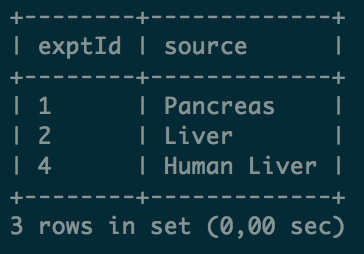
\includegraphics[scale=0.7]{Q1.png}
\centering
\end{figure}


\pagebreak

\textbf{Q2. Get 5 \textit{GenBank} ids and corresponding \textit{descriptions}.}

\color{blue}
\begin{verbatim}
mysql>	 SELECT gbId, description FROM Descriptions LIMIT 5;
\end{verbatim}
\color{black}

\begin{figure}[H]
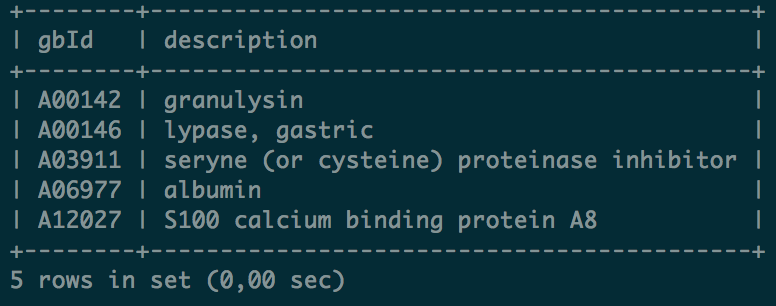
\includegraphics[scale=0.7]{Q2.png}
\centering
\end{figure}


\textbf{Q3. What is the purpose of this query?}

\begin{verbatim}
mysql>	 SELECT count(*) from LocusLinks;
\end{verbatim}
\color{blue}
It counts the total number of entries in the table \textit{LocusLinks}.
\color{black}

\begin{figure}[H]
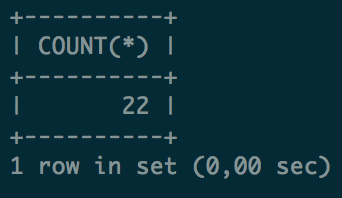
\includegraphics[scale=0.7]{Q3.png}
\centering
\end{figure}


\textbf{Q4. How many different \textit{Affy} ids are in the expression data?}

\color{blue}
\begin{verbatim}
mysql>	 SELECT COUNT(affyId) FROM Data;
\end{verbatim}
\color{black}

\begin{figure}[H]
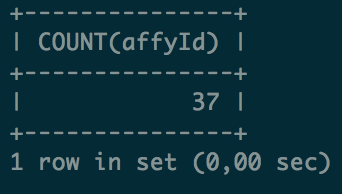
\includegraphics[scale=0.7]{Q4.png}
\centering
\end{figure}


\textbf{Q5. What is the expression level of \textit{Affy} id \textit{U95-32123\_at} in experiment number 1?}

\color{blue}
\begin{verbatim}
mysql>	 SELECT level FROM Data WHERE affyId="U95-32123_at" AND exptId=1;
\end{verbatim}
\color{black}

\begin{figure}[H]
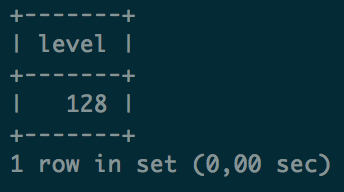
\includegraphics[scale=0.7]{Q5.png}
\centering
\end{figure}


\textbf{Q6. Find all the gene \textit{descriptions}, along with their \textit{GenBank} ids containing the word "\textit{Human}"?}

\color{blue}
\begin{verbatim}
mysql>	 SELECT * FROM Descriptions WHERE description LIKE "%Human%";
\end{verbatim}
\color{black}

\begin{figure}[H]
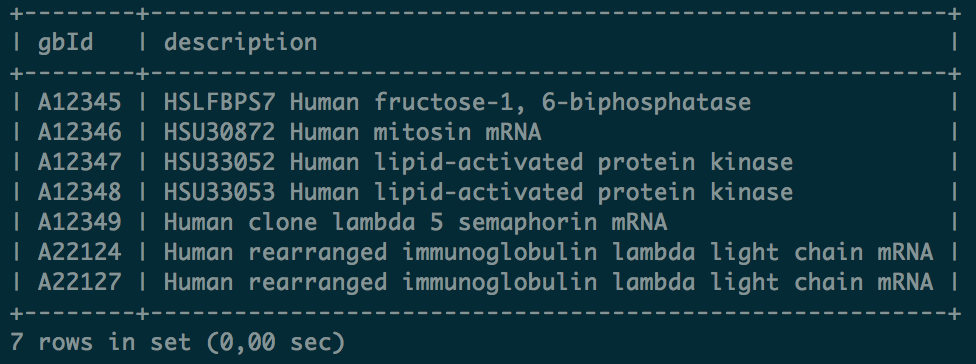
\includegraphics[scale=0.7]{Q6.png}
\centering
\end{figure}


\textbf{Q7. What \textit{Gene Ontology descriptions} (and corresponding \textit{accession}) contain the phrase "\textit{protein kinase}"? Answer should be provided in ascending order of accessions.}

\color{blue}
\begin{verbatim}
mysql>	 SELECT * FROM GO_Descr WHERE description LIKE "%protein kinase%"
mysql>	 ORDER BY goAcc ASC;
\end{verbatim}
\color{black}

\begin{figure}[H]
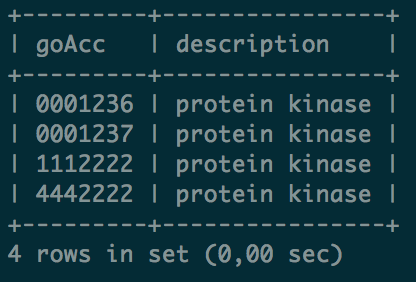
\includegraphics[scale=0.7]{Q7.png}
\centering
\end{figure}


\textbf{Q8. Which \textit{AffyId} of table \textit{Data} correspond to sequences in \textit{Targets} table with the phrase "\textit{kinase}" in their \textit{description}?}

\color{blue}
\begin{verbatim}
mysql>	 SELECT Data.affyId FROM Data, Targets, Descriptions
mysql>	 WHERE Data.affyId=Targets.affyId
mysql>	 AND Targets.gbId=Descriptions.gbId
mysql>	 AND Descriptions.description LIKE "%kinase%";
\end{verbatim}
\color{black}

\begin{figure}[H]

\includegraphics[scale=0.7]{Q8.png}
\centering
\end{figure}


\textbf{Use the following command:}

\begin{verbatim}
LOAD DATA INFILE `file.tsv' INTO TABLE Targets;
\end{verbatim}
 
 
\textbf{To add a new entry in \textit{Descriptions} with the string "\textit{kinase}" and the \textit{gbId="M18228"}. Now repeat the query again.}

\color{blue}
Repeating the same query again is still showing 0 results. There is an \textit{affyId} corresponding to the \textit{gbId} that we have introduced (\textit{M18228}), but that \textit{affyId} is not in the \textit{Data} table.
\color{black}

\begin{figure}[H]

\includegraphics[scale=0.7]{Q8.png}
\centering
\end{figure}


\textbf{Q9. Get two \textit{affyId}, \textit{uId} and \textit{descriptions} in \textit{LocusDescr} in reverse alphabetical order of \textit{descriptions}.}

\color{blue}
\begin{verbatim}
mysql>	 SELECT Targets.affyId, UniSeqs.uId, LocusDescr.description
mysql>	 FROM LocusDescr, LocusLinks, Targets, UniSeqs 
mysql>	 WHERE UniSeqs.gbId=LocusLinks.gbId AND Targets.gbId=LocusLinks.gbId
mysql>	 AND LocusLinks.linkId=LocusDescr.linkId ORDER BY description DESC LIMIT 2;
\end{verbatim}
\color{black}
 
\begin{figure}[H]
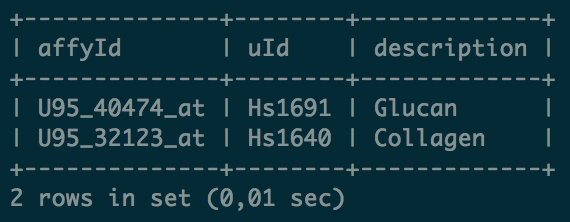
\includegraphics[scale=0.7]{Q9.png}
\centering
\end{figure}


\textbf{Q10. How would you find the average expression level of each experiment in \textit{Data}?}

\color{blue}
\begin{verbatim}
mysql>	 SELECT exptId, AVG(level) FROM Data GROUP BY exptId;
\end{verbatim}
\color{black}

\begin{figure}[H]
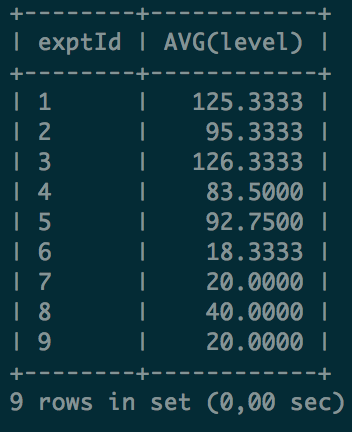
\includegraphics[scale=0.7]{Q10.png}
\centering
\end{figure}


\pagebreak

\textbf{Q11. What is the average expression level of each array probe (\textit{affyId}) across all experiments?}

\color{blue}
\begin{verbatim}
mysql>	 SELECT affyId, AVG(level) FROM Data GROUP BY affyId;
\end{verbatim}
\color{black}

\begin{figure}[H]
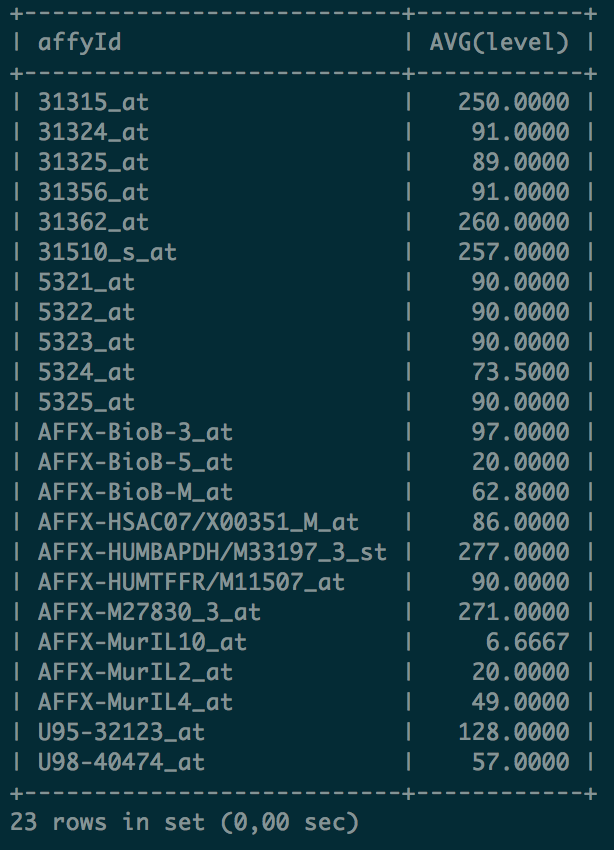
\includegraphics[scale=0.7]{Q11.png}
\centering
\end{figure}


\textbf{Q12. What is the purpose of the following query?}
\begin{verbatim}
mysql>	 SELECT Data.affyId, Data.level, Data.exptId, DataCopy.affyId,
mysql>	 DataCopy.level, DataCopy.exptId
mysql>	 FROM Data, Data DataCopy
mysql>	 WHERE Data.level > 10 * DataCopy.level
mysql>	 AND Data.affyId=DataCopy.affyId
mysql>	 AND Data.affyId LIKE "AFFX%''
mysql>	 LIMIT 10;
\end{verbatim}

\color{blue}
From the table called "\textit{Data}" it takes the entries with an \textit{affyId} beginning with the string "\textit{AFFX}". Then, it selects those whose levels are ten times higher than the levels of other experiments of the same \textit{affyId}. Finally, it shows up the first ten matches.
\color{black}

\begin{figure}[H]
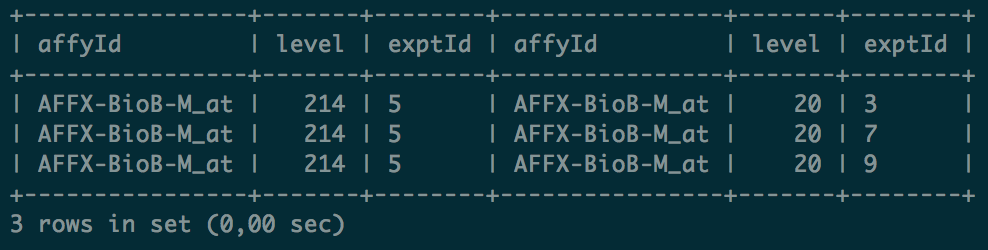
\includegraphics[scale=0.7]{Q12.png}
\centering
\end{figure}


\textbf{Q13. Write a query to provide three different descriptions for all \textit{gbId} in table \textit{Targets}.}

\color{blue}
There are four tables containing descriptions. Therefore, there are 4 possible combinations and 4 possible outputs, depending on which three tables are chosen (\textit{Descriptions}, \textit{LocusDescr}, \textit{GO\_Descr} or \textit{UniDescr}).
One of the possibilities is the following one:
\begin{verbatim}
mysql>	 SELECT Targets.gbId, Descriptions.description AS General_Description,
mysql>	 LocusDescr.description AS Locus_Description,
mysql>	 GO_Descr.description AS GO_Description
mysql>	 FROM Targets, Descriptions, LocusDescr, LocusLinks, GO_Descr, Ontologies
mysql>	 WHERE Descriptions.gbId=Targets.gbId
mysql>	 AND Targets.gbId=LocusLinks.gbId AND LocusLinks.linkId=LocusDescr.linkId
mysql>	 AND LocusLinks.linkId=Ontologies.linkId
mysql>	 AND Ontologies.goAcc=GO_Descr.goAcc;
\end{verbatim}
\color{black}

\begin{figure}[H]
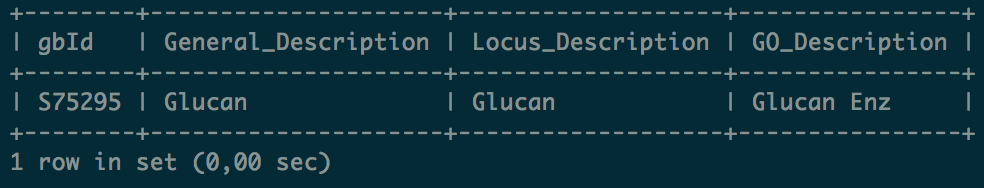
\includegraphics[scale=0.7]{Q13.png}
\centering
\end{figure}


\textbf{Q14. Write a query to provide all gene ontology (\textit{GO\_descr}) descriptions related with all species in table \textit{Species} sorted alphabetically and providing the first five results. Export the query to a tab-separated-file with the command:}

\begin{verbatim}
mysql>	 SELECT * FROM TABLE INTO OUTFILE 'data.out';
\end{verbatim}

\color{blue}
\begin{verbatim}
mysql>	 SELECT * FROM(
mysql>	 SELECT MY.species, GO_Descr.description FROM GO_Descr, (
mysql>	 SELECT LocusDescr.linkId, LocusDescr.species FROM LocusDescr
mysql>	 UNION
mysql>	 SELECT LocusLinks.linkId, Targets.species
mysql>	 FROM LocusLinks, Targets where Targets.gbId=LocusLinks.gbId
mysql>	 ) AS MY, Ontologies
mysql>	 WHERE Ontologies.linkId=MY.linkId AND GO_Descr.goAcc=Ontologies.goAcc
mysql>	 ORDER BY species ASC LIMIT 5
mysql>	 ) AS FINAL INTO OUTFILE '14.out';
\end{verbatim}
\color{black}

\begin{figure}[H]
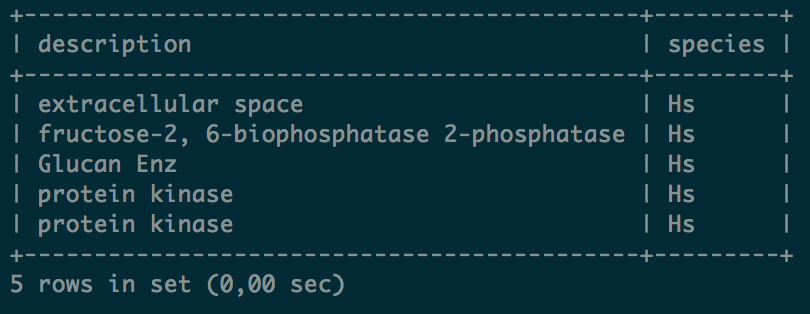
\includegraphics[scale=0.7]{Q14.png}
\centering
\end{figure}


\end{document}